\documentclass[a4paper]{article}
% \begin{minipage}[b]{Xcm}
% first column
% \end{minipage} \hfill \begin{minipage}[b]{Ycm}
% second column
% \end{minipage}
% [b] : to align in the bottom
% {Xcm} and {Ycm} : the width of each column (instead of {Xcm} we can use \textwidth)
% \textwidth : the width of the general page

% Preamble
\usepackage{graphicx}
\begin{document}
\begin{figure}[!h]
    \begin{minipage}[b]{0.5\textwidth}  % 30 percent of the page
        La imagen de la derecha muestra en icosaedro junto con un dodecaedra (figura central), los satélites son un 
        icosaedro, un dodecaedro y un tetraedo. Las figuras fueron generadas con {\sc Mathematica} y maquilladas con 
        {\it Inkscape}
        \end{minipage}
        \hfill
        \begin{minipage}[b]{0.5\textwidth}  % 60 percent of the page
			\begin{center}
				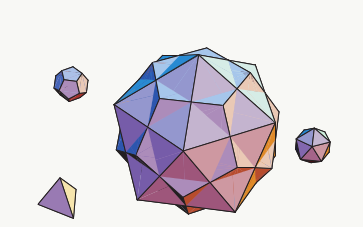
\includegraphics[scale=0.5]{ML.png}
				\caption{Polyedra}
			\end{center}
    \end{minipage}
\end{figure}

% Using the command \raisebox{distance}{text}
% {distance} : The distance to be araised respect to the second argument. If it's negative the text goes down.
\end{document}
